 %\subsection{1d tqft}
 %definition: $F \colon \mathsf{Bord} _1 \to \mathsf{Vect} $. $n$ is the top dimension (eg zero manifolds with 1-manifold bordisms). unoriented case. what kind of data do we get? in $\mathsf{Bord} _1$, objects are compact 0-manifolds, eg a finite collection of points. $F(\bullet)=V$. $F\left(\coprod_k \bullet\right)\simeq  F(\bullet)\otimes F(\bullet) \otimes \cdots \otimes F(\bullet)=V^k$ (symmetric monoidal). 

 %What about bordisms? Bordisms go left to right. line between points is identity. so it gets sent to identity, therefore $\id_V$. circle maps $\O \to \O$, $\O \mapsto k$, identity is $\O \colon \O \to \O$. so $F(S^1 ) \colon k \to k $, or a scalar, say $\lambda$. $S^1  \to \lambda$, then $S^1 \amalg S^1  \mapsto \lambda^2$ (composition). main tool: cut things up. write circle as composition of two intervals($\O \to  \bullet \amalg \bullet \to \O$). Theory $F$ associates to bilinear form $V \otimes V \to k$ (pairing). This is symmetric, flip by $\sigma$ in the bordism category (clearly diffeomorphic). evaluation and coevaluation.
 %\begin{claim}
     %This bilinear form is non-degenerate. Eg $\langle v,w \rangle =0$ for all $w$ implies $v=0$. (to be proved)
 %\end{claim}
 %look at coevaluation. through $F$ gets mapped to  $k \to V \otimes V$. in general, for $k \to U, 1 \mapsto u$, then linearly extend. $\alpha  \mapsto  \alpha u$. $\Hom(k,U)\simeq  U$ is determined by $1$. Therefore $f \colon k \to U \mapsto f(1)$. so for $k \to V\otimes V, 1 \mapsto \sum _i^m  v_i  \otimes w_i $ (haven't picked a basis, just a general element).

%relation in $\mathsf{Bord} _1$: glue evaluation and coevaluation in a zig-zag, id to ev to coev to id. equivalent to id. functor preserves compositions, functor has to satisfy the same relation.

%{\color{red}todo: what relation does this imply about $F(ev)$ andd $F(coev)$? write out the condition in terms of the two maps $\langle v,w \rangle $ and $ 1 \mapsto \sum _i  ^m v_i  \otimes w_i $. then we can compute the value of a circle} 
 

%{\color{red}todo:basis for a tensor product write down proof. natural transformation of symmetric monoidal functors.}  examples: set under $\amalg,\O$, top under $\amalg$. bord, $\amalg, \O$. symmetric monoidal structure on bord, think about it.

%equality vs natural isomorphism (homotopy). strict 2-category


\section{Topological quantum field theory} 
In the same way we study abstract groups via their representations, in the same way we study bordism categories via representations.
\begin{definition}[]
    Fix $n \in \Z ^{\geq 0}$. Let $C$ be a symmetric monoidal category. An $ \mathbf n$\textbf{-dimensional topological quantum field theory with values in} $\mathbf C$ is a symmetric monoidal functor \[
    F \colon \mathrm{Bord}_{\langle n-1,n \rangle } \to  C.
    \] 
\end{definition}
Recall that homology theory gives us symmetric monoidal functors $H_q \colon \left( \mathsf{Top} ,\amalg \right)  \to \left( \mathsf{Ab} ,\oplus \right) $ for $q \in \Z ^{\geq 0}$. One should think of the direct sum as \emph{classical}; for \emph{quantum} field theories we will use instead the tensor product. In vague terms, ``quantization'', the passage from classical to quantum, is a sort of exponentiation turning sums to products.
\begin{example}
    Typical ``linear'' choices for $C$ are:
    \begin{enumerate}[label=(\roman*)]
    \setlength\itemsep{-.2em}
\item the symmetric monoidal category $\left( \mathsf{Vect} _k,\otimes \right) $ of vector spaces over a field $k$,
\item the symmetric category $({}_R \mathsf{Mod} ,\otimes) $ of left modules over a commutative ring $R$,
\item the symmetric monoidal category $\left( \mathsf{Ab} ,\otimes \right) $ of abelian groups under the tensor product.
    \end{enumerate}
    We could also take the codomain to be a bordism category, which is decidedly nonlinear. For example, if $M$ is a closed $k$-manifold, then there is a symmetric monoidal functor $- \times M \colon \mathsf{Bord} _{\langle n-1,n \rangle } \to \mathsf{Bord} _{\langle n+k-1,n+k \rangle }$. Let $F \colon \mathsf{Bord} _{\langle n+k-1,n+k \rangle } \to $ be any $\left( n+k \right) $-dimensional TQFT, then composition with $- \times M$ gives an $n$-dimensional TQFT, the \textbf{dimensional reduction of} $\mathbf F$ \textbf{along} $\mathbf M$. \[
    \mathsf{Bord} _{\langle n-1,n \rangle } \xrightarrow{- \times M}  \mathsf{Bord} _{\langle n+k-1,n+k \rangle } \xrightarrow{F} C
    \] 
\end{example}
\begin{remark}
    If $M$ is a closed oriented $n$-manifold, we can view $M$ as a bordism $\O^{n-1}\to \O^{n-1}$, determining a morphism in $\mathsf{Bord} _{\langle n-1,n \rangle }$. If $Z$ is an $n$-dimensional TQFT, then $M$ determines a map $Z(M) \colon Z(\O) \to Z(\O)$. Now $Z$ preserves unit objects as a tensor functor, that is, $Z(\O)$ is \emph{canonically} isomorphic to the base field $k$. Consequently, we can think of $Z(M)$ as an element of the endomorphism ring $\Hom _{\mathsf{Vect} _k}(k,k)$, that is, an element of $k$. So the functor $Z$ assigns a \emph{number} to every closed oriented manifold of dimension $n$.
\end{remark}

\subsection{TQFTs as a symmetric monoidal category}
Fix $B= \mathsf{Bord} _{\langle n-1,n \rangle }$ and a symmetric monoidal category $C$. We explain that TQFTs $F \colon B \to C$ are objects in a symmetric monoidal category, with morphisms being symmetric monoidal natural transformations. The monoidal product of theories is defined by 
\begin{align*}
    (F_1 \otimes F_2)(Y) &= F_1(Y) \otimes F_2(Y) \\
    (F_1 \otimes F_2)(X) &= F_1(X) \otimes F_2(X)
\end{align*}for all objects $Y \in B$ and morphisms $(X \colon Y_0 \to Y_1) \in B$. The tensor unit $\mathbf 1$ is the trivial theory \[
1(Y)=1_C, \quad 1(X)=\id_{1_C}
\] for all $Y \in B$ and $(X \colon Y_0 \to Y_1) \in B$. The symmetric monoidal categories of TQFTs is then denoted as \[
\mathrm{TQFT}_n =\mathrm{TQFT}_n [C]=\Hom ^{\otimes}\left( \mathsf{Bord} _{\langle n-1,n \rangle },C \right) .
\] 
\begin{example}
    Suppose $\eta \colon \mathbf 1 \to \mathbf 1$ in $\mathrm{TQFT}_n $. Then for all $Y \in \mathsf{Bord} _{\langle n-1,n \rangle }$, we have $\eta(Y) \in  C(1_C,1_C) = \mathrm{End}(1_C)$. If $C= \mathsf{Ab} $, then $\mathrm{End}(1_C)= \Z$, so $\eta$ is a numerical invariant of closed $(n-1)$-manifolds. Furthermore if $X \colon Y_0 \to Y_1$ then by naturality we find that $\eta(Y_0)=\eta(Y_1)$. This shows that $\eta$ factors down to a homomorphism of monoids \[
        \eta \colon \Omega_{n-1}  \to \mathrm{End}(1_C).
    \] Now every element of $\Omega_{n-1}$ is invertible ($Y\amalg Y=\O$), so the image of $\eta$ consists of invertible elements. We say, simply, that $\eta$ is invertible. {\color{red}todo:related to assigning each manifold a number?} idea: $\eta $ is an $(n-1)$ diemnsional theory, assigning numbers to $(n-1)$ manifolds, preserved by equivalence class, bordism invariant.
\end{example}
\begin{theorem}
    A morphism $(\eta \colon F \to G) \in \mathrm{TQFT}_n $ is invertible, and $\mathrm{TQFT}_n $ is a groupoid.
\end{theorem}
The two statements are equivalent.
\begin{namedthing}{Central problem} 
    Given a dimension $n$ and a codomain category $C$ we can ask to ``compute'' the groupoid  $\mathrm{TQFT}_n [C]$. This is a vague problem whose solution is an equivalent groupoid which is ``simpler'' than the groupoid of topological quantum field theories. It has a nice answer when $n=1$. In the oriented case it is a generalization of the theorem that $\Omega_0^{\mathrm{SO}}$ is the free abelian group with a single generator $\mathrm{pt}_+$. There is also a nice answer in the oriented case for $n=2$.
\end{namedthing}
\subsection{Finiteness}
\begin{prop}
    Let $F \colon \mathsf{Bord} _{\langle n-1,n \rangle } \to \mathsf{Vect_{\C}} $ be a TQFT. Then for all $Y \in \mathsf{Bord} _{\langle n-1,n \rangle }$ the vector space $F(Y)$ is finite dimensional.
\end{prop}
\begin{figure}[H]
\centering
 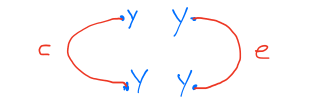
\includegraphics[width=0.3\linewidth]{figures/evcoev.png}
 \caption{Evaluation and coevaluation} 
 \label{evcoev} 
\end{figure}
\begin{figure}[H]
\centering
 \includegraphics[width=0.3\linewidth]{figures/sdiagram.png}
 \caption{The S-diagram} 
 \label{sdiagram} 
\end{figure}
\begin{proof}
    Fix $Y \in \mathsf{Bord} _{\langle n-1,n \rangle }$ and let $V=F(Y)$. Let  $c \colon \O ^{n-1} \to Y \amalg Y$ and $e \colon Y\amalg Y \to \O^{n-1}$ be the bordisms in \cref{evcoev}. The manifold $Y$ is depicted as a point, and each bordism has underlying manifold $[0,1] \times Y$. The composition depicted in \cref{sdiagram} is diffeomorphic to the identity bordism $\id _Y \colon Y \to Y$, which maps to $\id_V \colon V \to V$ under $F$. OTOH, the compositon maps to \[
        V \xrightarrow{\id_V \otimes F(c)} V\otimes V\otimes V\xrightarrow{F(e)\otimes \id_V} V.
    \] Let the value of  $F(c) \colon \C \to V\otimes V$ on $1 \in \C$ be $\sum _i  v_i '\otimes v_i ''$ for some finite set of vectors $v_i ', v_i '' \in V$. Then equating with the identity map, we get that for all $\xi \in V$, $\xi =\sum _i e(\xi ,v_i ')v_i ''$, and so $v_i ''$ spans $V.$ Then $V$ is finite dimensional, and we are done.
\end{proof}
It is clear to see that $F(c) \colon \C \to V\otimes V$ and $F(e) \colon V\otimes V \to \C$ are inverse bilinear forms, since both their compositions are diffeomorphic to the identity. Explicitly, $F(c) \colon 1 \mapsto  \sum _i  v_i '\otimes v_i ''$, and sending this through $F(e)$ results in 1.

\subsection{Duality}
\begin{definition}[]
    Let $C$ be a symmetric monoidal cateogry and $y \in C$. 
    \begin{enumerate}[label=(\roman*)]
    \setlength\itemsep{-.2em}
\item \textbf{Duality data} for $y$ is a triple of data $(y ^{\vee},c,e)$ in which $y^{\vee}$ is an object of $C$ and $c,e$ are morphisms $c \colon 1_C \to y\otimes y^{\vee}, e \colon y ^{\vee} \otimes y\to 1_C$. We require that the compositions \[
y \xrightarrow{c\otimes\id_y} y\otimes y^{\vee}\otimes y\xrightarrow{\id_y \otimes e} 
\] and \[
y ^{\vee}\xrightarrow{\id_{y^{\vee}} \otimes c} y ^{\vee}\otimes y \otimes y ^{\vee}\xrightarrow{e \otimes \id_{y ^{\vee}} } y ^{\vee}
\] be identity maps. If duality data exists for $y$, then we say that $y$ is \textbf{dualizable}.
\item A \textbf{morphism of duality data} $(y^{\vee},c,e) \to (\widetilde y ^{\vee},\widetilde e,\widetilde e)$ is a morphism $y^{\vee}\xrightarrow f \widetilde {y ^{\vee}} $ such that the diagrams \[
\begin{tikzcd}
                                                  &  & y\otimes y^{\vee} \arrow[dd, "\id_Y\otimes f"] \\
1_C \arrow[rru, "c"] \arrow[rrd, "\widetilde c"'] &  &                                                \\
                                                  &  & y \otimes \widetilde{y^{\vee}}                
\end{tikzcd}
\] and \[
\begin{tikzcd}
 y^{\vee}\otimes y \arrow[dd, "f\otimes \id_Y"'] \arrow[rrd, "e"] &  &     \\
                                                                  &  & 1_C \\
\widetilde{y^{\vee}}\otimes y \arrow[rru, "\widetilde e"']        &  &    
\end{tikzcd}
\] commute. $c$ is called \textbf{coevaluation} and $e$ is called \textbf{evaluation}. 
    \end{enumerate}
\end{definition}
We now express the uniqueness of duality data. We cannot say there is a unique object as duality data is an object in a category, however, we do have the strongest form of uniqueness possible in a category: duality data is unique up to unique isomorphism.
\begin{definition}[]
    Let $C$ be a category.
    \begin{enumerate}[label=(\roman*)]
    \setlength\itemsep{-.2em}
\item If for each pair $y_0,y_1 \in C$ the hom-set $C(y_0,y_1)$ is either empty or contains a unique element, we say that $C$ is a \textbf{discrete groupoid} . {\color{red}todo:what about $y_0\neq y_1$ aren't there two choices? not equivalent to objects (only identity map)} 
\item If for each pair $y_0,y_1 \in C $ the hom-set $C(y_0,y_1)$ has a unique element, we say that $C$ is \textbf{contractible}. {\color{red}todo:check: contractible $\subseteq $ discrete groupoids}   

    \end{enumerate}
\end{definition}
A discrete groupoid is equivalent to a set. A contractible groupoid is equivalent to a category with one object and one morphism, the categorical analog of a point. We prove this second assertion.
\begin{proof}
    Let $G$ be a contractible groupoid. Consider a functor $F \colon G \to \mathrm{pt}$, where $g_i  \mapsto  \mathrm{pt}$ for every $g_i  \in G$ and $(g_i \xrightarrow{ij}g_j ) \mapsto \id_{\mathrm{pt}} $ for every morphism $ij \in \mathrm{Mor}(G)$. There is only one $d \in D$ so essential surjectivity is clear. In the same way, every pair of elements only has one morphism between them, so this functor is well-defined and a bijection (the target category only has one morphism as well, the identity $\id_{\mathrm{pt}}$). So $F$ is essentially surjective and fully faithful, and we are done. {\color{red}todo:check} 

    The reason why this argument fails for discrete groupoids is that \emph{for every} $c_1,c_2 \in C$, there has to be a bijection of hom sets onto its image. Sometimes $\Hom(g_1,g_2)$ will be empty in a discrete groupoid, hence there is no bijection $\O \to \{*\} $.
\end{proof}
\begin{prop}
    Let $C$ be a symmetric monoidal category and $y \in C$. Then the category of duality data for $y$ is either empty or contractible.
\end{prop}
\begin{proof}
    {\color{red}todo:} 
\end{proof}
\begin{definition}[]
    Let $y_0,y_1 \in C$ be dualizable objects in a symmetric monoidal category and $f \colon y_0 \to y_1$ a morphism. The \textbf{dual morphism}  $f ^{\vee} \colon  y_1 ^{\vee} \to y_0^{\vee}$ is the composition \[
    y_1 ^{\vee}\xrightarrow{\id _{y_1^{\vee}}\otimes c_0} y_1 ^{\vee}\otimes y_0 \otimes y_0 ^{\vee}\xrightarrow{\id_{y_1^{\vee}}\otimes f \otimes \id_{y_0 ^{\vee}} } y_1 ^{\vee }\otimes y_1 \otimes y_0 ^{\vee}\xrightarrow{e_1 \otimes \id _{y_0 ^{\vee}}} y_0^{\vee}
    \] 
\end{definition}
\begin{ex}
   For $C= \mathsf{Vect} $, let $T \colon M \to N$ be a linear map.
\end{ex}
